\begin{figure}
    \centering
    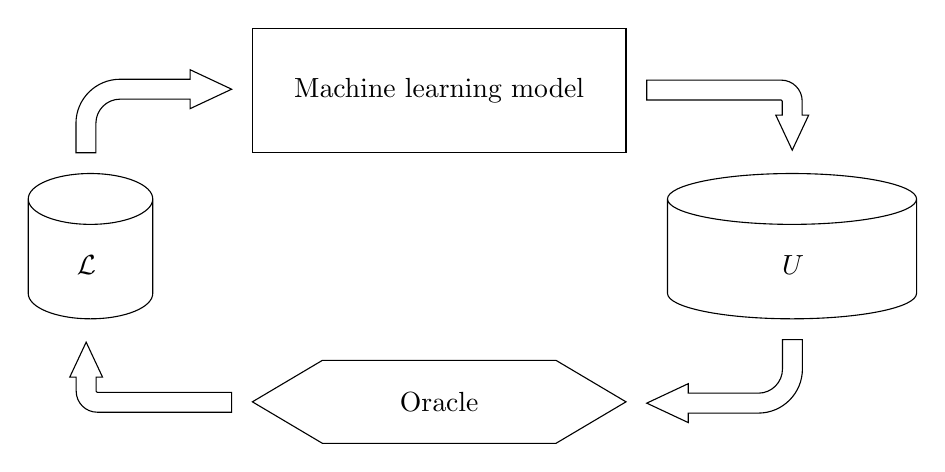
\begin{tikzpicture}[x=0.75pt,y=0.75pt,yscale=-1,xscale=1]
        %Flowchart: Magnetic Disk [id:dp9287936135344942] 
        \draw   (82,122.25) -- (82,167.75) .. controls (82,174.52) and (68.57,180) .. (52,180) .. controls (35.43,180) and (22,174.52) .. (22,167.75) -- (22,122.25)(82,122.25) .. controls (82,129.02) and (68.57,134.5) .. (52,134.5) .. controls (35.43,134.5) and (22,129.02) .. (22,122.25) .. controls (22,115.48) and (35.43,110) .. (52,110) .. controls (68.57,110) and (82,115.48) .. (82,122.25) -- cycle ;
        %Flowchart: Magnetic Disk [id:dp374407561883777] 
        \draw   (450,122.25) -- (450,167.75) .. controls (450,174.52) and (423.14,180) .. (390,180) .. controls (356.86,180) and (330,174.52) .. (330,167.75) -- (330,122.25)(450,122.25) .. controls (450,129.02) and (423.14,134.5) .. (390,134.5) .. controls (356.86,134.5) and (330,129.02) .. (330,122.25) .. controls (330,115.48) and (356.86,110) .. (390,110) .. controls (423.14,110) and (450,115.48) .. (450,122.25) -- cycle ;
        %Flowchart: Preparation [id:dp06966809995247569] 
        \draw   (130,220) -- (163.75,200) -- (276.25,200) -- (310,220) -- (276.25,240) -- (163.75,240) -- cycle ;
        %Bend Arrow [id:dp5182616743082409] 
        \draw   (395,190) -- (395,204.17) .. controls (395,215.91) and (385.48,225.43) .. (373.75,225.43) -- (340,225.43) -- (340,230) -- (320,220.63) -- (340,211.25) -- (340,215.83) -- (373.75,215.83) .. controls (380.18,215.83) and (385.4,210.61) .. (385.4,204.17) -- (385.4,190) -- cycle ;
        %Bend Arrow [id:dp8578173985872724] 
        \draw   (120,225) -- (55.24,225) .. controls (49.65,225) and (45.11,220.47) .. (45.11,214.88) -- (45.11,208.13) -- (42,208.13) -- (49.91,191.25) -- (57.82,208.13) -- (54.71,208.13) -- (54.71,214.88) .. controls (54.71,215.17) and (54.94,215.41) .. (55.24,215.41) -- (120,215.41) -- cycle ;
        %Flowchart: Process [id:dp753078500376894] 
        \draw   (130,40) -- (310,40) -- (310,100) -- (130,100) -- cycle ;
        %Bend Arrow [id:dp18815347737102261] 
        \draw   (45,100) -- (45,85.83) .. controls (45,74.09) and (54.52,64.58) .. (66.26,64.58) -- (100,64.58) -- (100,60) -- (120,69.38) -- (100,78.75) -- (100,74.17) -- (66.26,74.17) .. controls (59.82,74.17) and (54.6,79.39) .. (54.6,85.83) -- (54.6,100) -- cycle ;
        %Bend Arrow [id:dp0737210580323302] 
        \draw   (320,65) -- (384.76,65) .. controls (390.35,65) and (394.89,69.53) .. (394.89,75.13) -- (394.89,81.88) -- (398,81.88) -- (390.09,98.75) -- (382.18,81.88) -- (385.29,81.88) -- (385.29,75.13) .. controls (385.29,74.83) and (385.06,74.59) .. (384.76,74.59) -- (320,74.59) -- cycle ;
        
        % Text Node
        \draw (50,154) node   {$\mathcal{L}$};
        % Text Node
        \draw (390.5,154) node   {$U$};
        % Text Node
        \draw (220,220) node  [align=left] {Oracle};
        % Text Node
        \draw (220,70) node  [align=left] {Machine learning model};
    \end{tikzpicture}
    \caption{The active learning cycle. At the beginning, only a small number of labeled instances can be used by the learner (labeled training set \(\mathcal{L}\): the learner proceeds in a standard (semi-)supervised way, building a model starting from \(\mathcal{L}\). Then, the algorithm can query an oracle requesting labels for a number of examples: usually, there is a huge amount of unlabeled examples to choose from --- i.e., the unlabeled training set \(\mathcal{U}\). The new labeled instances are added to the set \(\mathcal{L}\), and the cycle starts again.}
    \label{active_learning_cycle}
\end{figure}